\chapter{Bilder}
\label{bewegungsprofile_anhang}

\textbf{Bewegungsprofile geloggt über die Echtzeitschnittstelle \& geplottet in Matlab}

\begin{figure}[H]
  \centering
    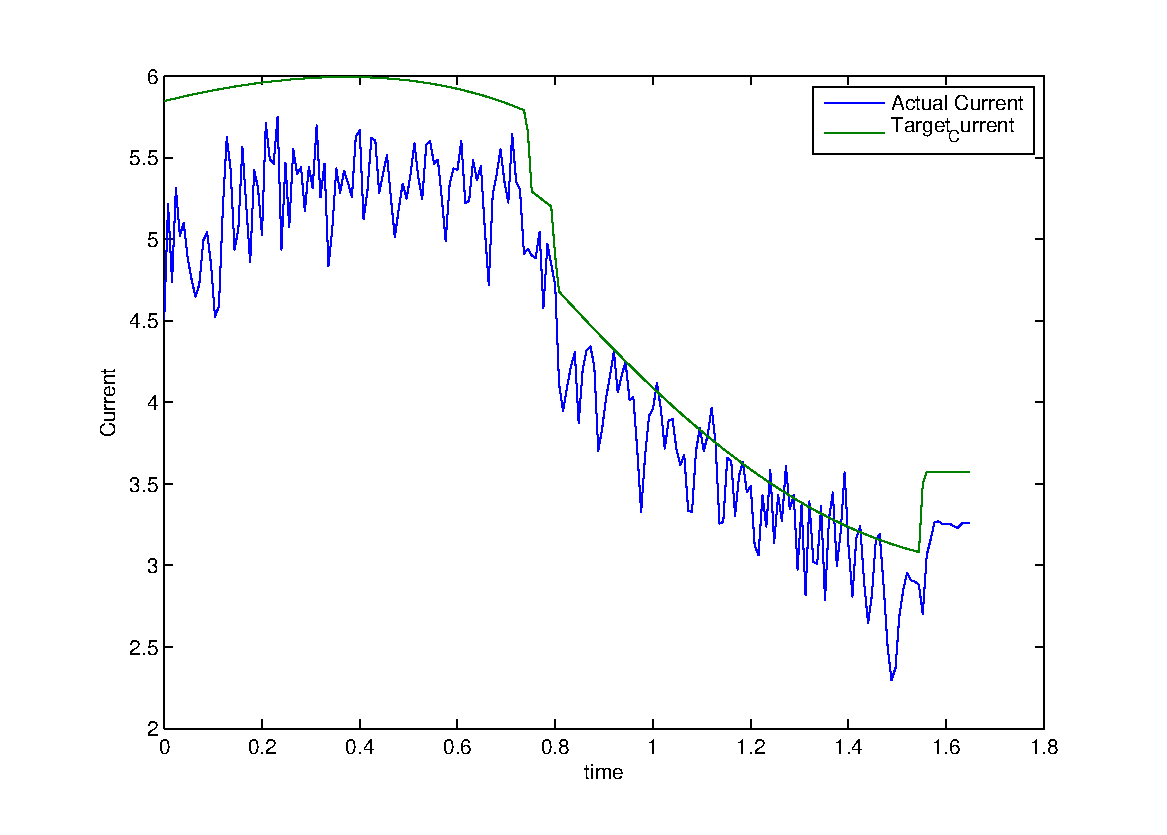
\includegraphics[width=1\textwidth]{pic/joint1_polyscope_current.eps}
      \caption[Soll-und Ist-Werte der Stromstärke wärend der Bewegung des 2.Gelenks mit Polyscope]{Abbildung zeigt den berechneten Offset des Ist-Wertes.}
      \label{fig:current_profile_joint1_rci}
\end{figure}

\begin{figure}[H]
  \centering
    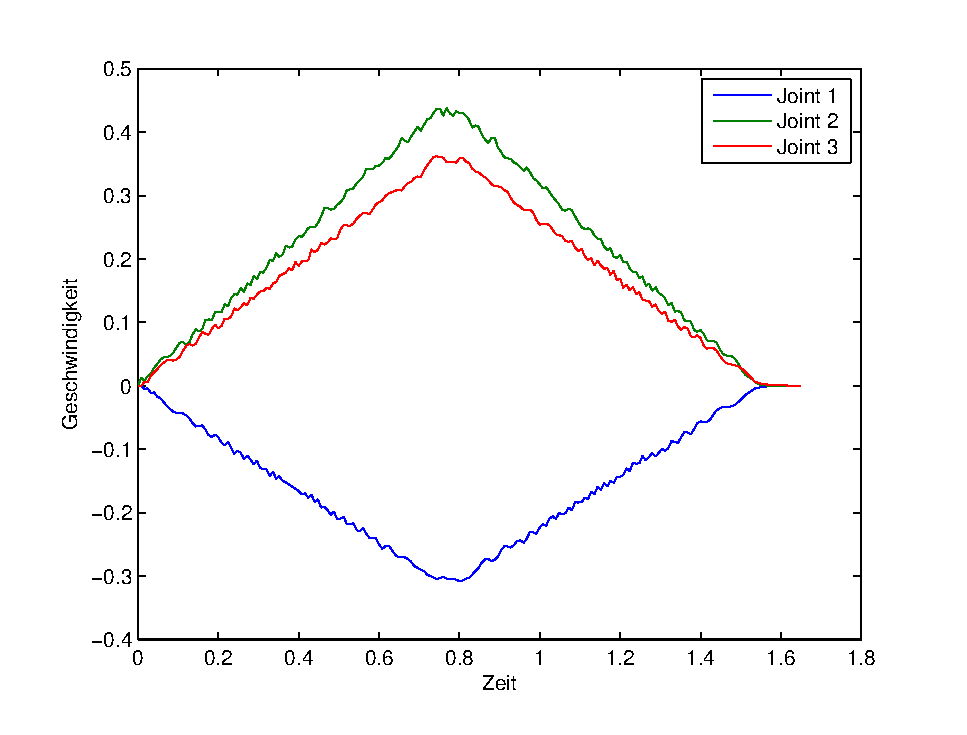
\includegraphics[width=1\textwidth]{pic/velocity_profile_polyscope.eps}
      \caption[Geschwindigkeitsprofil wärend der Bewegung der Gelenke 1-3 mit Polyscope]{Abbildung zeigt das Geschwindigkeitsprofil der Gelenke 1-3, während eines Bewegungsprofils mit Polyscope. Profil wurde mit der Echtzeitschnittstelle geloggt}
      \label{fig:velocity_joints_rci}
\end{figure}

\begin{figure}[H]
  \centering
    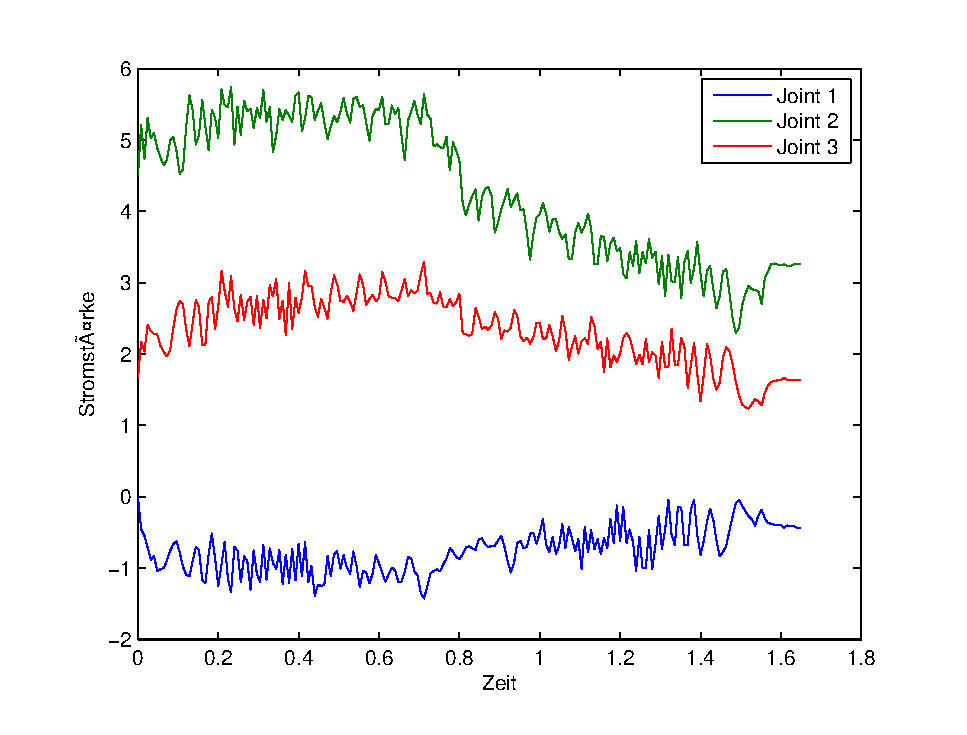
\includegraphics[width=1\textwidth]{pic/current_profile_polyscope.eps}
      \caption[Stromstärke wärend der Bewegung der Gelenke 1-3 mit Polyscope]{Abbildung zeigt die Stromstärke der drei Gelenke 1,2 und  während eines Bewegungsprofils, das wurde mit der Echtzeitschnittstelle geloggt wurde.}
      \label{fig:acceleration_profile_rci}
\end{figure}

\begin{figure}[H]
  \centering
    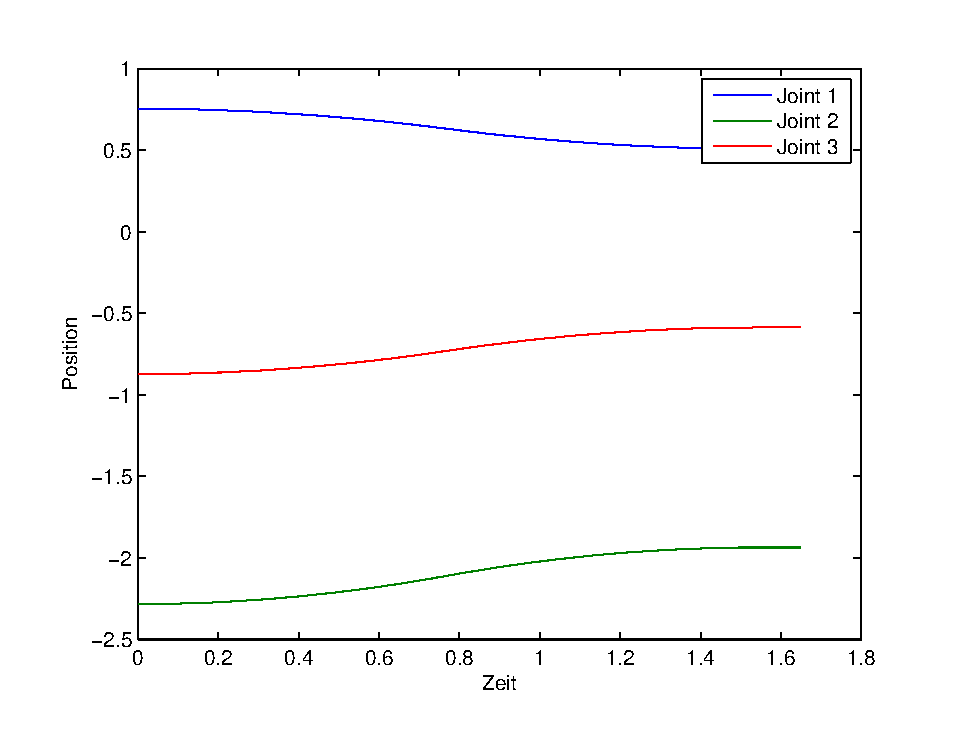
\includegraphics[width=1\textwidth]{pic/position_profile_polyscope.eps}
      \caption[Position wärend der Bewegung der Gelenke 1-3 mit Polyscope]{Abbildung zeigt die Position der Gelenke 1-3, während eines Bewegungsprofils mit Polyscope. Profil wurde mit der Echtzeitschnittstelle geloggt}
      \label{fig:position_joints_rci}
\end{figure}

\textbf{Bewegungsprofile geloggt in der C-API}

\begin{figure}[H]
  \centering
    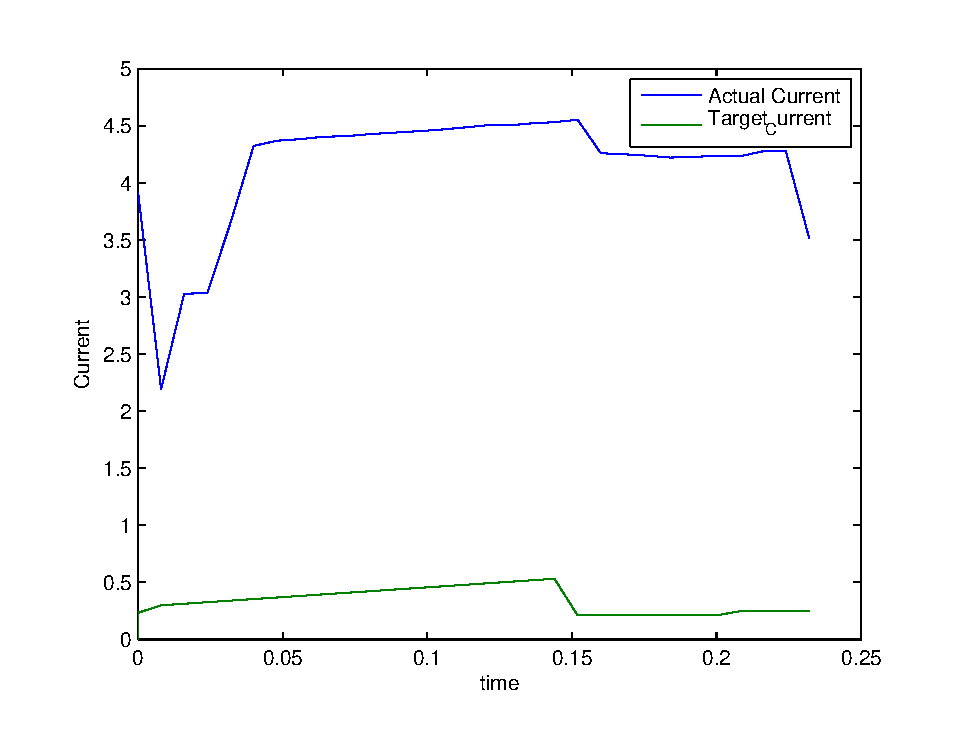
\includegraphics[width=1\textwidth]{pic/joint1_current_capi.eps}
      \caption[Soll-und Ist-Werte der Stromstärke des 2.Gelenks]{Abbildung zeigt die Soll-Werte und Ist-Werte der Stromstärke des 2.Gelenks, kurz vor dem Sicherheitsstopp}
      \label{fig:joint_1_position_capi}
\end{figure}

\textbf{Bilder vom Roboter}

\begin{figure}[H]
  \centering
    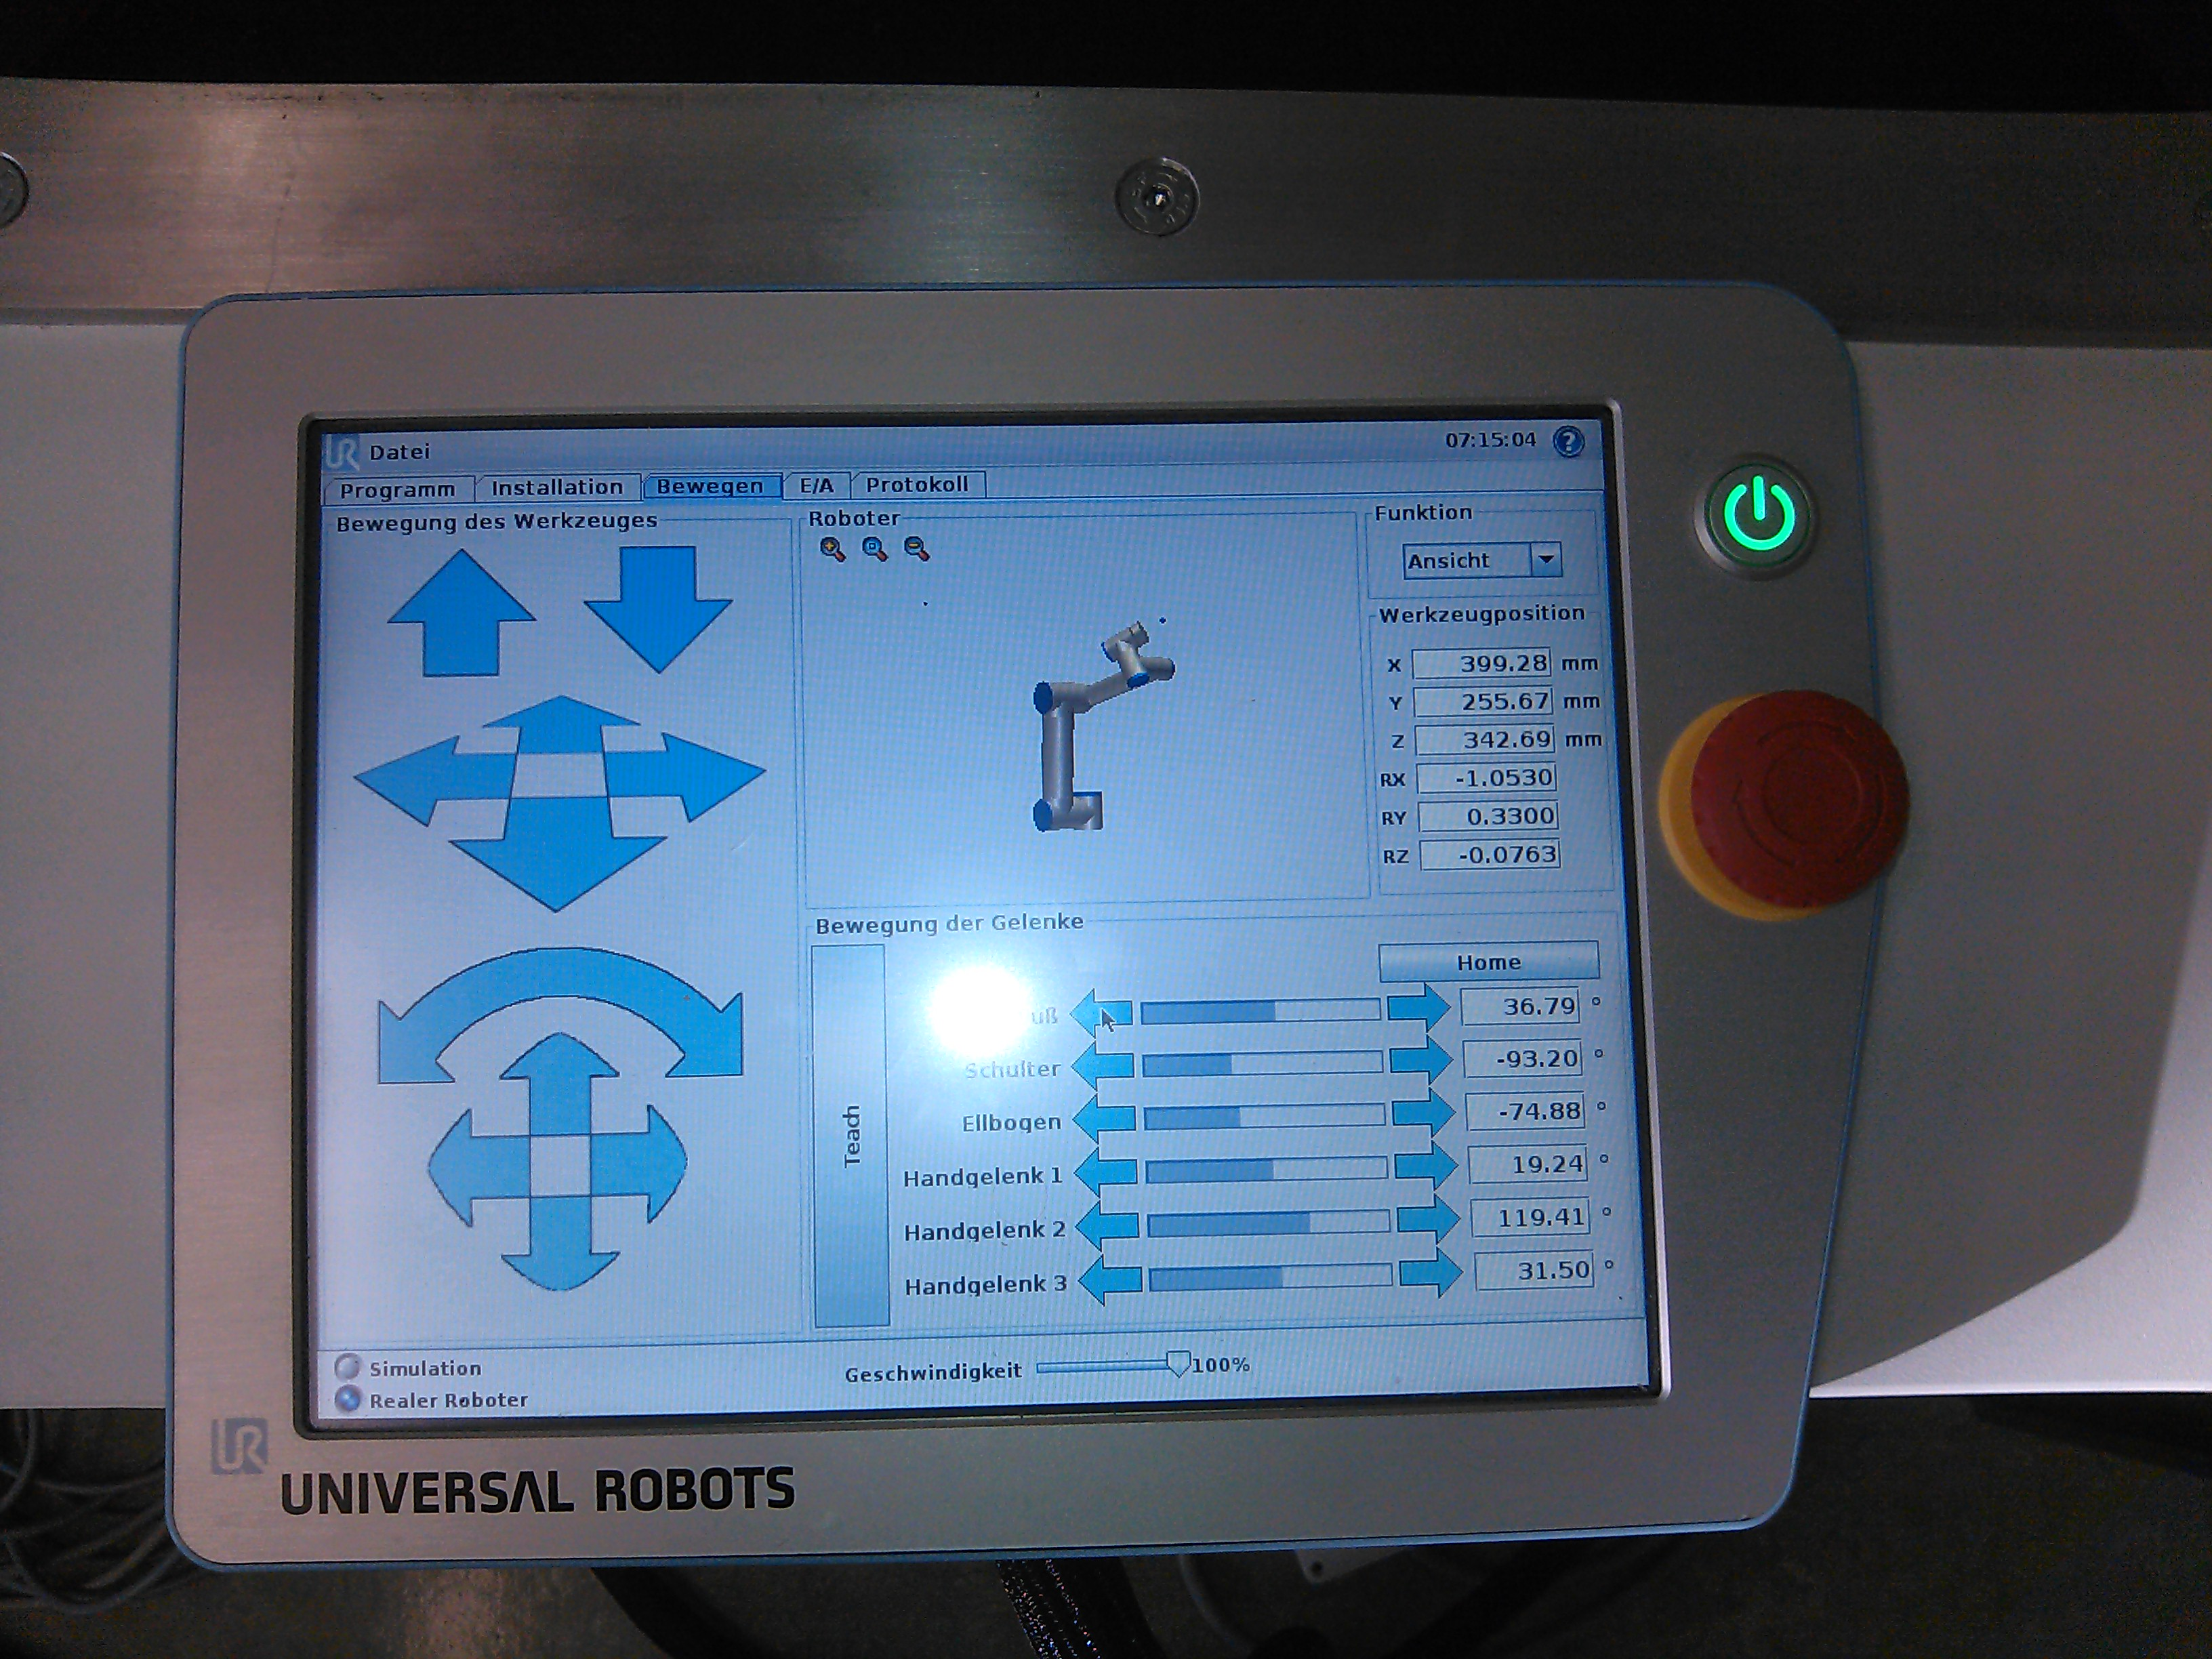
\includegraphics[width=1\textwidth]{pic/tablet.jpg}
      \caption[Soll und Ist Werte der Position des 2.Gelenks]{}
      \label{fig:tablet_picture}
\end{figure}


\chapter{Quellcode}
\label{quellcode}

\section{Speichern der Daten über \ac{TCP/IP} in der Datenbank}
\label{save_data_tcp_code_gru}

\begin{lstlisting}
#!/usr/bin/env python2.7

from my_utils import connection, Player, get_ip
import socket
import signal
import sys
import os

class SaveDataInterface():
    def __init__(self, interface="localhost"):
        self.__run_flag=False
        self.interface = interface
        self.socket=socket.socket(socket.AF_INET, socket.SOCK_STREAM)
        ip = get_ip(interface)
        if ip is None:
            ip="127.0.0.1"
        else:
            ip = get_ip(interface)
        port = 8000
        self.socket.setsockopt(socket.SOL_SOCKET, socket.SO_REUSEADDR, 1)
        try:
            self.socket.bind((ip, port))
            print "server is listen on %s:%d" %(ip, port)
            self.socket.listen(1)
        except socket.error, e:
            print(e[0])
            self.socket.close()
            self.socket=None

    def run(self):
        self.__run_flag=True
        # print("starting send interface waiting for queue")
        while self.__run_flag:
            if self.socket is not None:
                conn, addr = self.socket.accept()
                conn.settimeout(2)
                print "client connected: {0}".format(addr)
                player=None
                while self.__run_flag:
                    msg = self.read_from_socket(conn)
                    if msg is not None:
                        if msg == "new_patient":
                            # print("wait for new patient name")
                            name = self.read_from_socket(conn)
                            player = connection.Player()
                            player.name = name.rstrip()
                            player.save()
                        elif msg == "load_patient":
                            print("wait for patient name")
                            name = self.read_from_socket(conn)
                            player = connection.Player.find_one({'name': name.rstrip()})
                            if player is not None:
                                print("send %s"%"1".encode('ascii'))
                                print("positions %s"%("(%s)"%player.start_pos[1:-1]).encode('ascii'))
                                conn.send("(1)".encode('ascii'))
                                conn.send(("(%s)"%player.start_pos[1:-1]).encode('ascii'))
                            else:
                                conn.send("(0)".encode('ascii'))
                        elif msg == "set_patient_data":
                            # print("wait for player data")
                            start_position = self.read_from_socket(conn)
                            player.start_pos=start_position.rstrip()
                        else:
                            print("recieved unknown command")
                    else:   
                        break
                conn.close()

        self.socket.close()
        return 0

    # This Function reads from the Socket conn the next msg checks for errors
    def read_from_socket(self, conn):
        msg = None
        while self.__run_flag:
            try:
                msg = conn.recv(1024)
            except socket.timeout, e:
                err = e.args[0]
                # this next if/else is a bit redundant, but illustrates how the
                # timeout exception is setup
                if err == 'timed out':
                    # print 'recv timed out, retry later'
                    continue
                else:
                    print e
                    msg=None
            except socket.error, e:
                print e
                msg=None
            else:
                if len(msg) == 0:
                    msg=None
                    break
                else:
                    print msg
                    break
        return msg


sdi = SaveDataInterface(interface="eth0")

sdi.run()
\end{lstlisting}